\section{Professor}
\subsection{Dashboard}
Trang Dashboard giáng viên cung cấp một giao diện trực quan giúp điều hướng đến những trang khác một cách dễ dàng gồm các thành phần chính như sau:
\begin{itemize}
    \item Thống kê giảng viên:
    \begin{itemize}
        \item Hiển thị tổng số khóa học mà giảng viên quản lý: chuyển đến trang danh sách khóa học
        \item Tổng số sinh viên đang theo học trong các khóa học: chuyển đến trang tiến độ sinh viên trong khóa học
        \item Hiển thị tổng số bài giảng mà giảng viên đã thiết lập.
        \item Hiển thị tổng số bài tập đã được giao cho sinh viên: chuyển đến trang tạo bài tập.
    \end{itemize}
    \begin{figure}[H]
        \centering
        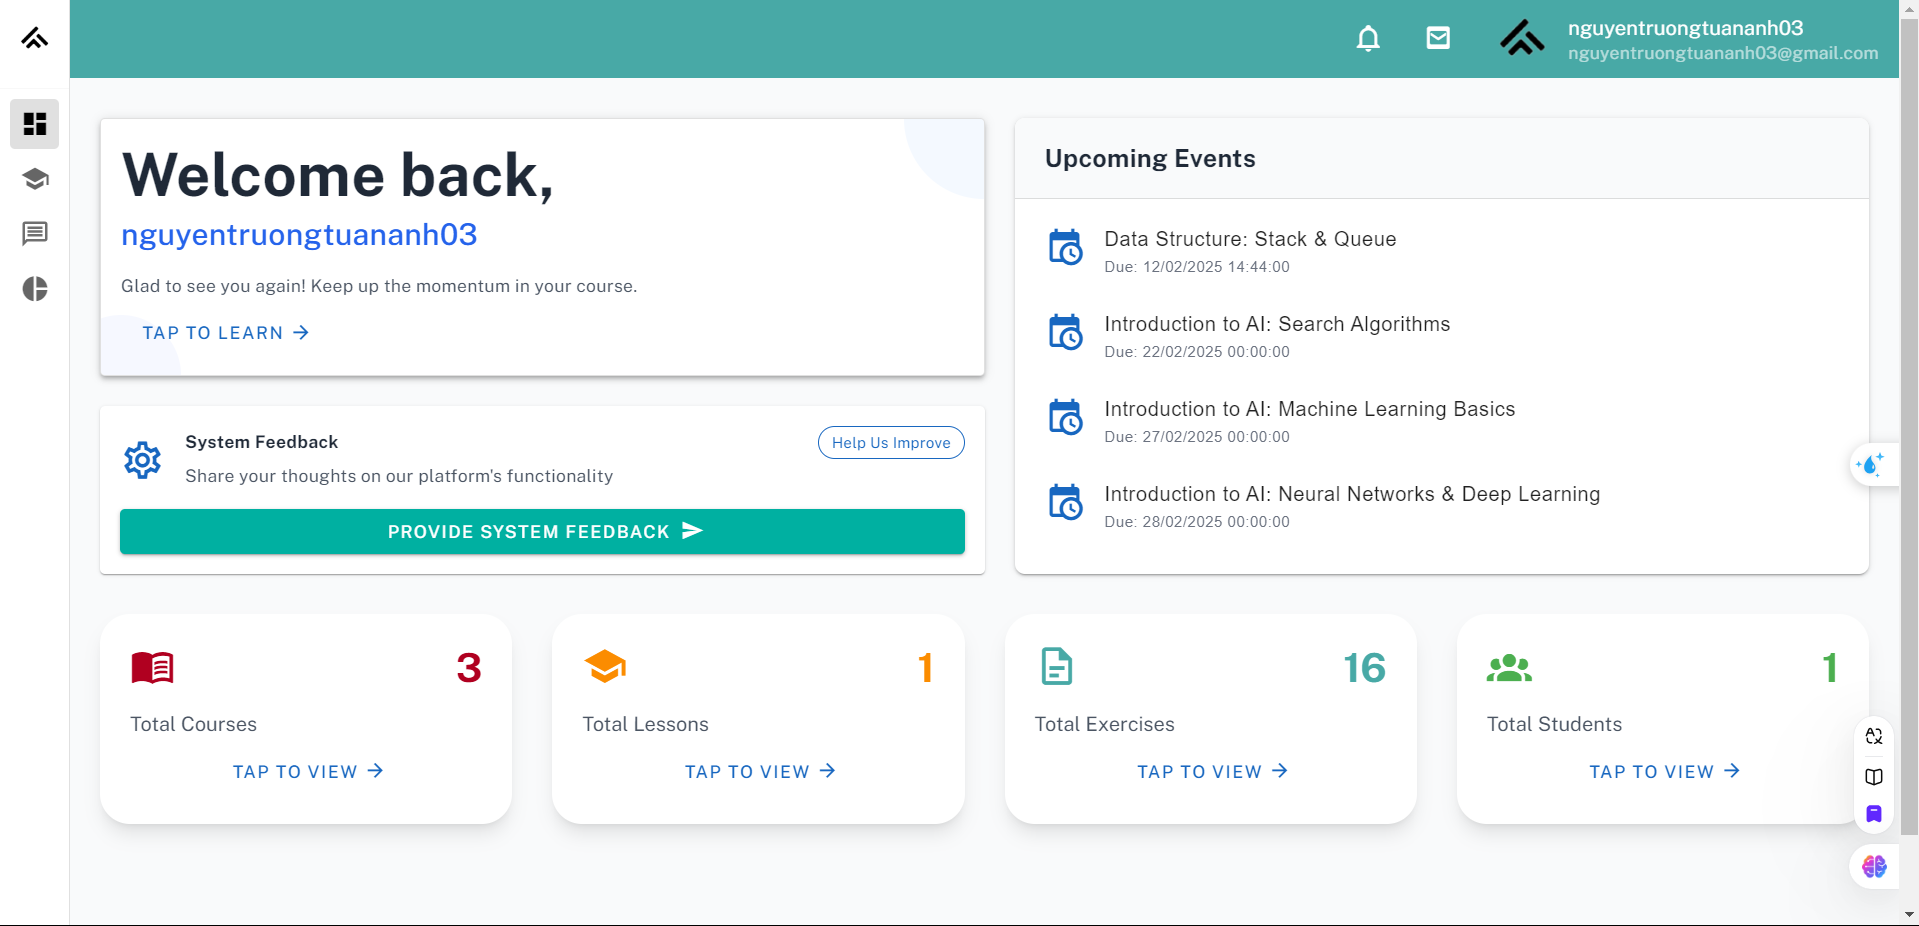
\includegraphics[width=0.8\linewidth]{images/dashboard_professor.png}
        \caption{Dashboard Professor}
        \label{fig:enter-label}
    \end{figure}
    \item Upcoming Events: hiển thị danh sách các sự kiện quan trọng sắp diễn ra mà giảng viên cần quan tâm (Hạn nộp bài tập, kỳ thi, sự kiện liên quan đến học viên)
    \item Gửi Feedback cho hệ thống: Giảng viên có thể gửi feedback về hệ thống qua một modal.
    \begin{figure}[H]
        \centering
        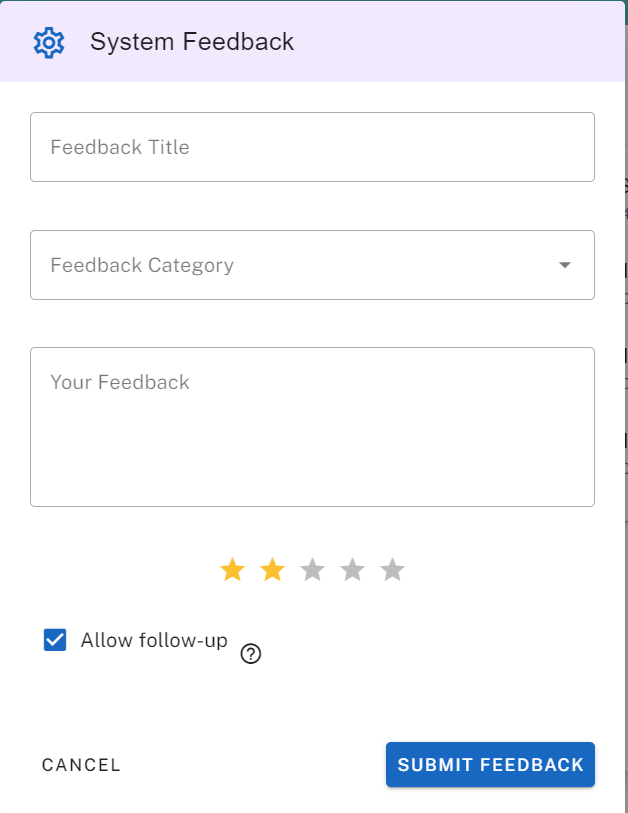
\includegraphics[width=0.3\linewidth]{images/modal_feedback.png}
        \caption{Modal Feedback}
        \label{fig:enter-label}
    \end{figure}
\end{itemize}
\subsection{My Course}
Trang My Course cung cấp danh sách các khóa học mà giảng viên phụ trách. Mỗi khóa học gồm các thông tin chi tiết như: tên khóa học, mã khóa học, sinh viên, learning outcomes, trạng thái khóa học, thời gian khóa học.
\begin{figure}[H]
        \centering
        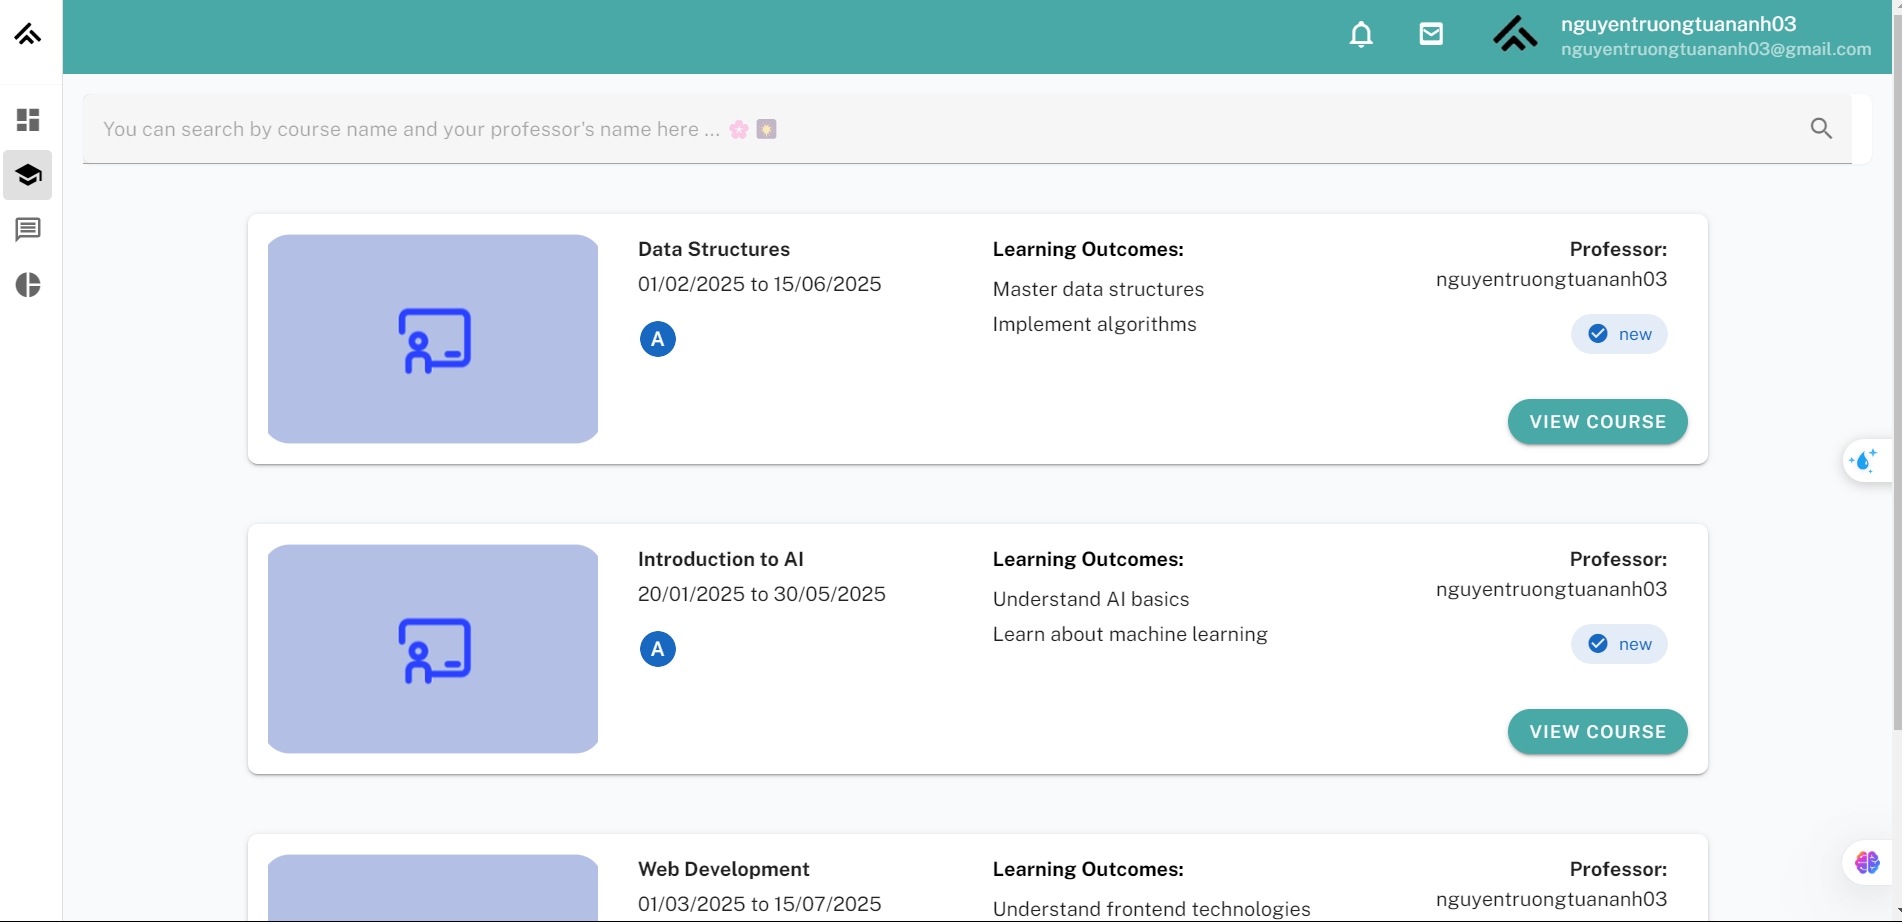
\includegraphics[width=0.8\linewidth]{images/course_professor.png}
        \caption{Professor: My Course}
        \label{fig:enter-label}
    \end{figure}
\subsection{Feedback Management}
Tính năng quản lý phản hồi giúp giảng viên theo dõi và phân tích ý kiến của sinh viên về khóa học.
\begin{itemize}
    \item Giảng viên có thể chọn một khóa học cụ thể từ danh sách các khóa học mà họ đang giảng dạy.
    \item Hệ thống sẽ hiển thị ra danh sách feedback gồm các thông tin: người gửi, tiêu đề phản hồi, mô tả, phân loại, rating.
    \begin{figure}[H]
        \centering
        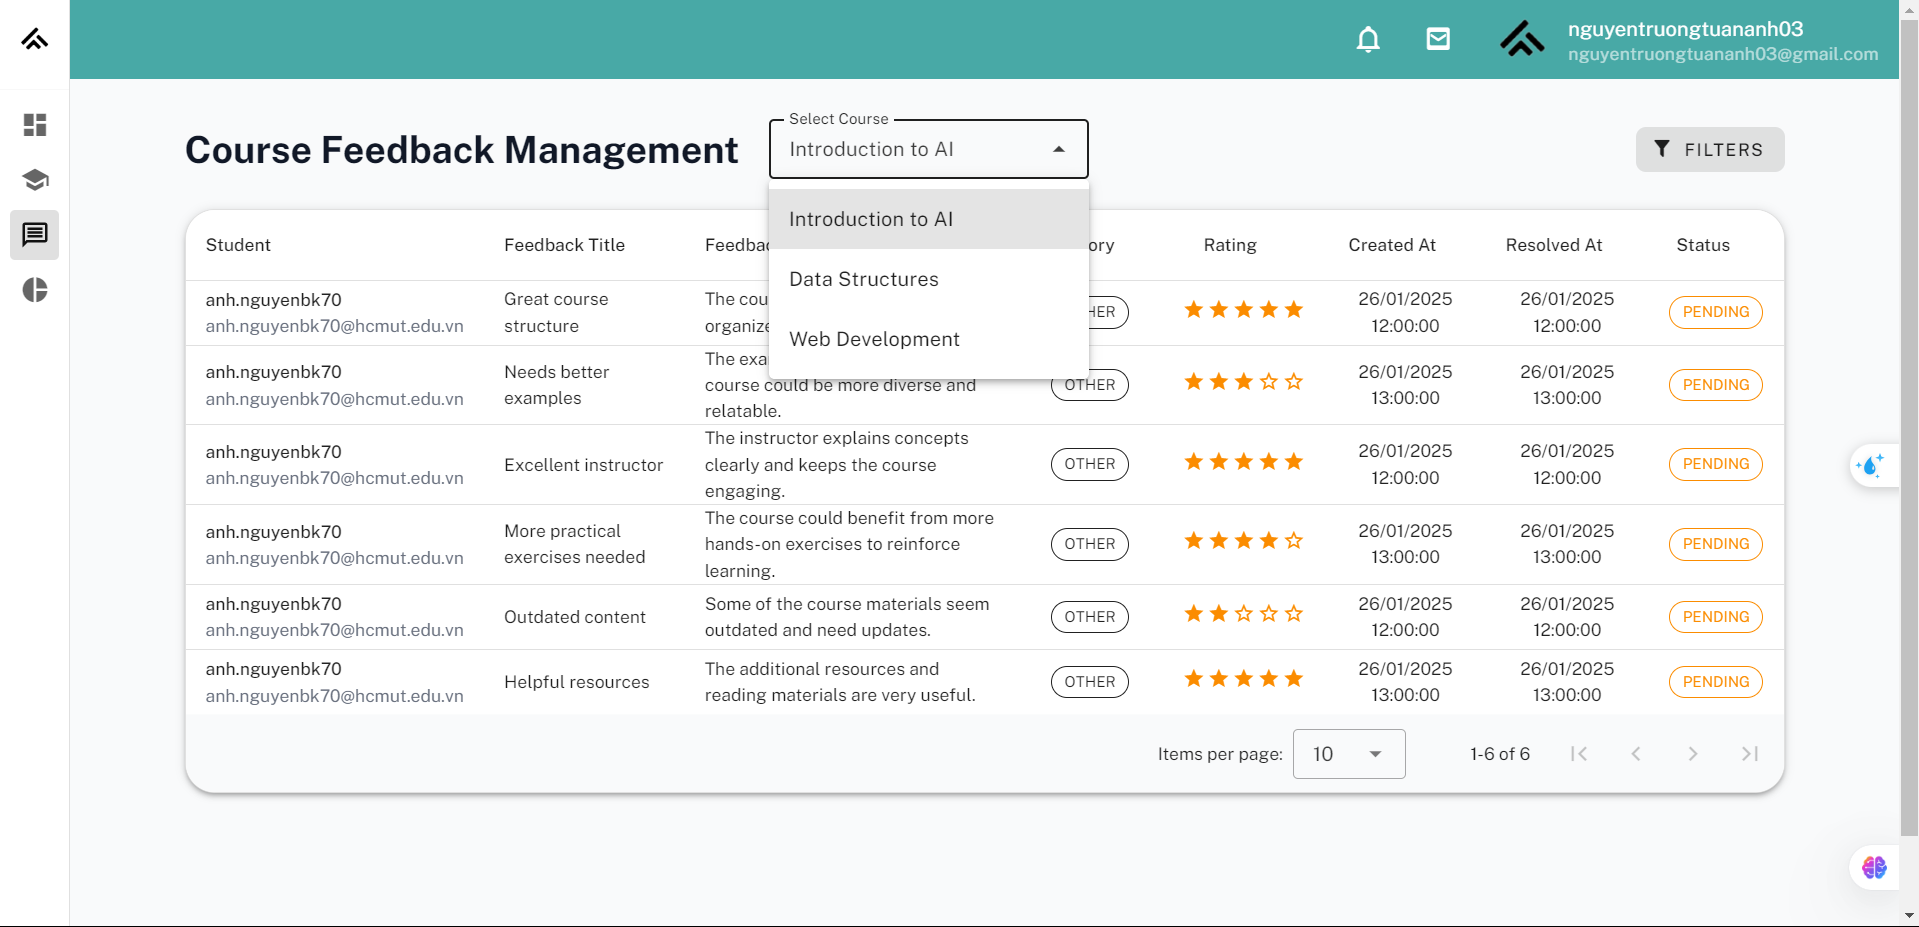
\includegraphics[width=0.8\linewidth]{images/feedback_professor.png}
        \caption{Professor: Feedback Management}
        \label{fig:enter-label}
    \end{figure}
\end{itemize}
\subsection{Progress Student}
Trang tiến độ này theo dõi tiến độ sinh viên giúp giảng viên đánh giá hiệu suất học tập của từng sinh viên trong khóa học
\begin{itemize}
    \item Tổng quan lớp học: điểm cao nhất, thấp nhất, trung bình điểm
    \item Tiến độ cá nhân: 
    \begin{itemize}
        \item Learning path cá nhân của sinh viên trong khóa học.
        \item Điểm số của từng bài kiểm tra và bài tập.
    \end{itemize}
    \item Chi tiết bài tập: Điểm của sinh viên trong bài tập, lời giải, lịch sử nộp bài và số lần thử lại.
\end{itemize}
 \begin{figure}[H]
        \centering
        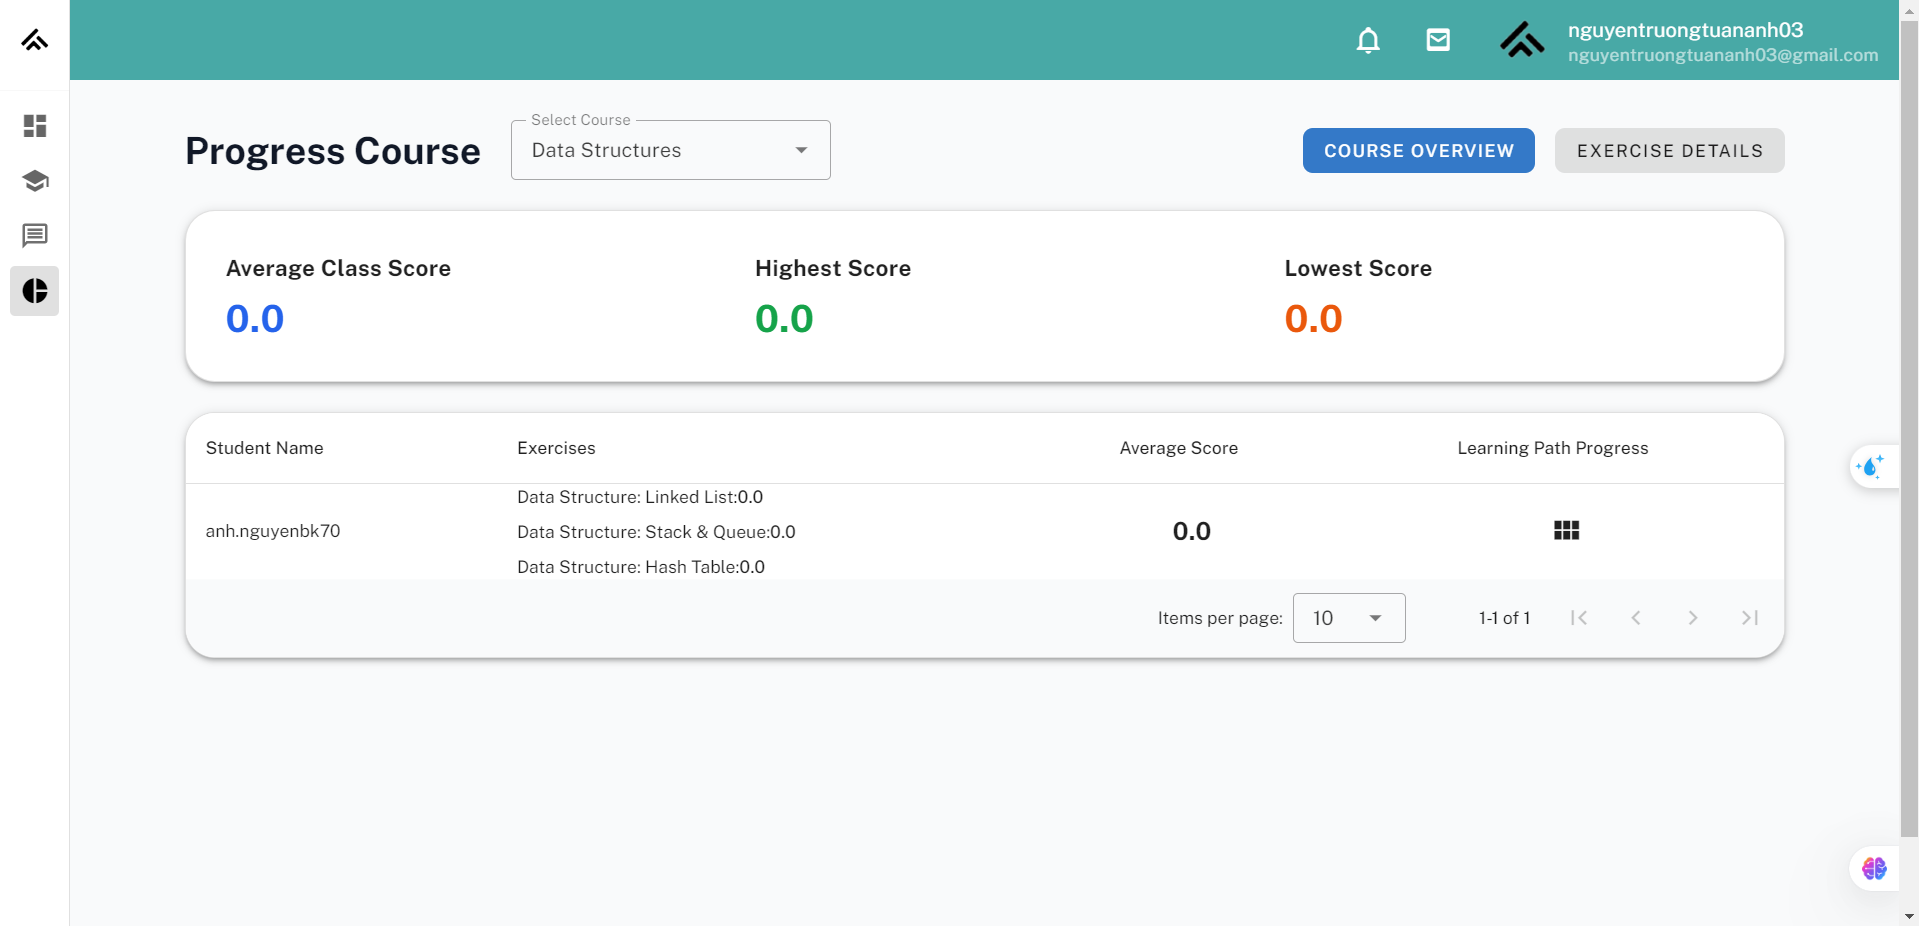
\includegraphics[width=0.8\linewidth]{images/progress_professor.png}
        \caption{Professor: Progress Student}
        \label{fig:enter-label}
    \end{figure}